\chapter{Non-Intrinsic Defects in PtSn\textsubscript{4}} \label{appen:non-intrinsic}
%todo: make differentiation between the non/intrinsic defect type and non/intrinsic defect number. meaning that there could be a defect type with both intrinsic and non-intrinsic origin
\begin{figure}
	\centering
	\includegraphics[width=0.8\textwidth]{Ch4_croissant.png}
	\caption[\textbf{Annihilation of two Sn$_1$ defects under STM topographies}]{\textbf{Annihilation of two Sn$_1$ defects under STM topographies}. The disappearance of both defects after repeated scanning suggests that Sn$_1$ defects can be dynamically created and annihilated, consistent with their interpretation as Frenkel pairs on the Sn site.}
	\label{fig:Ch4_croissantannihilation}
\end{figure}

In our experiment, we observed that the Sn$_1$ defect, located at the Sn site, is highly mobile under high scanning biases (exceeding 600 mV). Rotation of this defect is consistently seen in consecutive scans, as shown in Fig. \ref{fig:Ch4_rotationcroissant}, and instances of annihilation between two Sn$_1$ defects have also been documented (Fig. \ref{fig:Ch4_croissantannihilation} and Fig. \ref{fig:Ch4_rotationcroissant} b–c). These events demonstrate that Sn$_1$ defects can be both created and annihilated during scanning. This behavior also suggests that the origin of the Sn$_1$ defect could be a Frenkel pair on the Sn site.



\begin{figure}
	\centering
	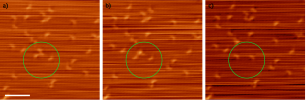
\includegraphics[width=0.8\textwidth]{Ch4_rotationcroissant.pdf}
	\caption[\textbf{Rotation and annihilation of Sn$_1$ defects during consecutive STM scans.}]{\textbf{Rotation and annihilation of Sn$_1$ defects during consecutive STM scans.}Highlighted regions (green circles) show rotational motion of individual Sn$_1$ defects followed by their eventual annihilation, further supporting their dynamic and non-intrinsic nature.}
	\label{fig:Ch4_rotationcroissant}
\end{figure}

While there is no direct evidence that Sn$_2$ and Sn$_3$ defects are non-intrinsic, their densities decrease systematically in samples with higher residual resistivity ratios (RRR) compared to those with lower RRR. This trend suggests that the presence of these defects may be influenced by sample quality or growth conditions, rather than being solely intrinsic to the material.

In conclusion, while STM studies capture intrinsic features of PtSn$_4$, experimental factors such as cleaving and scanning under high bias voltages can introduce non-intrinsic defects. Nonetheless, the fact that these defects can also exist intrinsically in bulk samples underscores the relevance of studying their properties and their influence on the material’s electronic behavior.


\chapter{Choice of $\epsilon$ in Numerical QPI Simulations} \label{app:epsilon}

In numerical simulations of quasiparticle interference (QPI) patterns on a square lattice, the parameter $\epsilon$, which enters as an $i\epsilon$ term in the Green's function, plays a pivotal role. Its selection is guided by both physical considerations and numerical stability requirements. In this appendix, we discuss the factors influencing the choice of $\epsilon$ and the trade-offs involved.

In a real material, quasiparticles have finite lifetimes due to various interactions, such as electron-electron, electron-phonon, and impurity scattering. The $i\epsilon$ term in the Green’s function is introduced as a phenomenological means to incorporate this finite lifetime. If experimental measurements or more detailed microscopic calculations suggest a particular scattering rate or linewidth, denoted by $\Gamma$, it is physically reasonable to choose $\epsilon \sim \Gamma$. For example, if the typical inverse lifetime is on the order of a few percent of the hopping parameter $t$, one might set $\epsilon \approx 0.01\,t$ to $0.05\,t$. A finite $\epsilon$ broadens sharp spectral features—such as van Hove singularities or defect-induced resonances—into Lorentzian peaks. However, if $\epsilon$ is too small, these peaks become excessively sharp, which may lead to numerical artifacts like spikes or convergence issues that do not accurately reflect the intrinsic physics. Conversely, an overly large $\epsilon$ may result in over-broadening, causing a loss of resolution in the QPI pattern.

The $i\epsilon$ prescription also has important implications for numerical stability and convergence. By moving poles away from the real axis, a finite $\epsilon$ prevents numerical divergences when evaluating the Green's function, particularly near band edges or resonances. In practice, when performing $k$-space integrations or Fourier transforms, the finite $\epsilon$ regularizes contributions from singular points, thereby enhancing the convergence of these integrals. Nevertheless, there is an inherent balance to be struck: while a smaller $\epsilon$ might capture finer spectral details, a slightly larger value is often required to ensure numerical stability. In some instances, adaptive schemes are used—starting with a larger $\epsilon$ for stability and then systematically reducing it while monitoring the convergence of the results.

Another important consideration is the relative scale of $\epsilon$ compared to other energy scales in the system. The dimensionless parameter in the Green’s function is frequently expressed as
\[
b = \frac{\omega + i\epsilon - E_0}{2t},
\]
which naturally suggests that $\epsilon$ should be small compared to the hopping parameter $t$ (and by extension, the bandwidth) so that it acts merely as a minor broadening factor rather than dominating the energy scale of the system. Additionally, in lattice simulations the momentum space is discretized, and a minimum broadening is required to mitigate aliasing or discretization errors. If $\epsilon$ is chosen too small, the computed density of states or QPI patterns may become overly sensitive to finite-size effects associated with the simulation grid.

Finally, practical considerations in QPI simulations often involve matching the simulation parameters to experimental observations. For instance, if scanning tunneling microscopy (STM) data show broadened features with a known linewidth, setting $\epsilon$ to mimic that broadening can enhance the fidelity of the simulation. It is also advisable to conduct sensitivity analyses by varying $\epsilon$ within a physically reasonable range. If the qualitative features of the QPI pattern remain robust under small changes in $\epsilon$, one can be more confident that the simulation is capturing the correct underlying physics.

In summary, the choice of $\epsilon$ in numerical QPI simulations is a balancing act. It must be small enough relative to the hopping parameter $t$ and the system's bandwidth to ensure that it only introduces a controlled broadening reflective of the finite quasiparticle lifetime, yet large enough to regularize singularities and smooth out discretization effects inherent in a finite simulation grid. By judiciously selecting $\epsilon$, one achieves both physical accuracy and numerical robustness in the simulation results.

\chapter{System parameter space of MC-SBD-STM}\label{appen:system_param}
To investigate the influence of system parameters—specifically the mini-loop number $N$ and the sparsity regularizer $\lambda$—on algorithmic performance, we constructed a benchmark testing pool comprising 12 synthetic \ac{STM} grid maps that emulate typical scanning conditions. One of these datasets was intentionally designed to represent an extremely challenging scenario, which we will highlight shortly. We then defined 15 distinct algorithmic configurations by combining $\text{mini-loop} \in {1, 3, 9}$ with $\lambda \in {0.01, 0.03, 0.1, 0.3, 0.5}$. Each of the 12 datasets was processed under all 15 configurations, resulting in a total of 180 algorithmic runs.

Each run was evaluated using two quantitative metrics: the kernel similarity and the activation map score, consistent with the definitions in Figure.\ref{fig:phase_space}. The results are visualized in two three-dimensional plots in Figure.\ref{fig:system_param}, where the $x$–$y$ plane represents the parameter space, and the $z$ axis encodes the metric value (higher values indicate better performance). Each sheet in these plots corresponds to one synthetic dataset and is color coded for clarity. The sheet exhibiting the poorest performance across both metrics is the same dataset (colored in red); this dataset corresponds to the intentionally challenging case and effectively delineates the algorithm’s performance boundary, as no tuning of the system parameters improves its results.

Qualitatively, by comparing panel a) and b), we observe that the sheets are noticeably flatter in kernel similarity, suggesting that the kernel similarity is largely insensitive to the choice of system parameters but remains sensitive to the condition of the input dataset. In contrast, the activation map score exhibits stronger dependence on the system parameters, making it a more appropriate metric to optimize the system parameter. To better visualize these dependencies, we projected the three-dimensional activation map results (Figure.\ref{fig:system_param} b) onto two dimensions and present them in Figure.\ref{fig:proj_system_param}. Panels a)–c) display projections onto the sparse regularizer $\lambda$ at different mini-loop numbers, with the $y$ axis showing the activation map score. Across all three mini-loop settings, we observe a trend of improved performance in the majority of datasets as $\lambda$ increases up to 0.3. More importantly, for $\text{mini-loop} = 1$ and $3$, $\lambda = 0.3$ yields near-optimal results, with the activation map score approaching unity. This can be seen more clearly in panel d), which isolates the case $\lambda = 0.3$. For comparison, panel e) shows the projection for $\lambda = 0.1$, which also demonstrates good performance for most datasets.

From this investigation, we determine the optimal range of system parameters as $\text{mini-loop} \in [1, 3]$ and $\lambda \in [0.1, 0.3]$. It is worth noting that the optimal sparse regularizer $\lambda$ reported here is valid only for two-dimensional input files. The dependence of the optimal $\lambda$ on three-dimensional inputs is discussed in detail in Section \ref{sec:guide}.  

\begin{figure}
	\includegraphics[width=\textwidth]{Appen_D_1.png}
	\centering
	\caption[\textbf{System parameter phase space}]{\textbf{System parameter phase space}}
	\label{fig:system_param}
\end{figure}

\begin{figure}
	\centering
	\includegraphics[width=\textwidth]{Appen_D_2.png}
	\caption[\textbf{2D projected view of system parameter space}]{\textbf{2D projected view of system parameter space}}
	\label{fig:proj_system_param}
\end{figure}

\chapter{Streak detection and correction}\label{appen:streak_detection}
Streaks in scanning tunneling microscopy (STM) data can originate from a variety of sources. One of the most common causes is tip change. In this scenario, the tip transitions from an initial state (state 1) to an altered state (state 2), resulting in a modified imaging response. This altered state typically persists for a finite duration before the tip reverts to its original state. The onset of a tip change can occur abruptly, often coinciding with the start of a new scan line in the slow-scan direction, or it may be triggered by a tip–surface interaction at specific surface features, such as defects. The transition between states leads to a pronounced change in image contrast, which manifests as the streak patterns commonly observed in both \ac{STM} topographies and grid maps.

Two principal effects arise from tip changes. The first is a baseline offset effect, where the tunneling current shifts between tip states 1 and 2. The second is a relative contrast effect, where the tip images surface features with a different relative intensity depending on its state. In most cases, the baseline offset dominates and is the primary focus of our correction algorithm.

To illustrate these effects, Figure \ref{fig:streak_1}, panel (a), shows a representative scan exhibiting tip changes. The data, taken from a ZrSiTe grid map with the fast-scan direction oriented vertically, displays streaks of darker contrast aligned with the fast-scan direction—signatures of transitions between tip states. The mean value of each column, plotted below panel (a), closely follows the bright–dark modulation in the image, confirming that the contrast changes are linked to tip-state transitions. Panel (b) plots these column means in greater detail, revealing a clear two-level distribution with mean currents of approximately $2\times10^{-13}$ A and $-5\times10^{-13}$ A, each corresponding to one of the two tip states. To further probe the effect of tip changes, we select two adjacent columns that straddle a tip-change event (indicated by the blue and purple arrows in panel a), corresponding to states 1 and 2, respectively. Their line profiles, shown in panel (c), highlight two key observations: (1) a clear global baseline offset between the two columns, and (2) the preservation of the periodic lattice corrugation pattern, demonstrating that the primary difference between tip states is a uniform current shift rather than a change in relative feature contrast.

In addition to full-column tip-state transitions, panel (b) also reveals columns with intermediate mean values that do not fall neatly into either tip state. For instance, column 13 has a mean current near zero (highlighted with a red dot and arrow in panel a), corresponding to a partial streak in the image. These partial streaks affect only a subset of rows within a column, making them challenging to correct with a simple column-wise leveling procedure. To address this, our algorithm detects the specific rows impacted by partial tip changes, allowing for more localized and accurate correction.

Streak identification involves two key elements: (1) determining the positions of the streak edges and (2) estimating the streak width along the horizontal direction. Edge detection is performed using the image Laplacian, which captures regions of rapid intensity change. The discrete horizontal Laplacian at pixel coordinates $(i,j)$ is defined as
$$L_{i,j} = I_{i,j-1} + I_{i,j+1} - 2I_{i,j}$$
where $I_{i,j}$ denotes the intensity at $(i,j)$. At locations where tip-state transitions cause abrupt changes in signal amplitude, this Laplacian yields large values, effectively marking the streak boundaries.

\begin{figure}
	\includegraphics[width=\textwidth]{AppenE_1.pdf}
	\centering
	\caption[\textbf{Illustration of tip-change–induced streaks and their correction challenge}]{\textbf{Illustration of tip-change–induced streaks and their correction challenge}(a) Representative slice of a ZrSiTe grid map with the fast-scan direction oriented vertically, showing dark streaks corresponding to tip-state transitions. The color strip below panel (a) plots the column-wise mean current, which exhibits alternating bright–dark modulation correlated with the streak pattern. (b) Detailed plot of the column means, revealing a clear two-level distribution with mean currents near $2\times10^{-13}$ A and $-5\times10^{-13}$ A, each associated with a distinct tip state. Column 13 (marked with a red arrow in panel a) shows an intermediate value, corresponding to a partial streak event. (c) Line profiles of two adjacent columns straddling a tip-change event (blue and purple arrows in panel a), demonstrating a global baseline offset between the two tip states while preserving the periodic lattice corrugation pattern.}
	\label{fig:streak_1}
\end{figure}

To detect streaks of varying widths, we employ a multi-scale Laplacian approach. Rather than relying solely on nearest neighbors, we compute Laplacian responses over multiple scales by varying the neighbor separation $n$:
$$L_n(i,j) = I_{i,j-n} + I_{i,j+n} - 2I_{i,j}$$
This calculation is performed for all $n < \text{max width}$, where max width specifies the largest expected streak width. The responses from all scales are then combined by taking the maximum absolute value at each pixel, producing a single composite Laplacian map. Thresholding this map yields a binary mask indicating streak locations. Figure \ref{fig:streak_2}b shows an example of such a mask (white pixels), which successfully identifies all streaks in the pre-processed image in panel (a).

Once identified, the streaked pixels are corrected iteratively, proceeding column by column from left to right. Each affected column—or partial column, in the case of partial streaks—is adjusted such that its mean value matches that of the nearest unperturbed column to its left for the corresponding rows. This process propagates across all subsequent columns, producing the corrected image shown in panel (e). For comparison, panel (f) displays the result of a conventional column-wise leveling approach, which fails to handle partial streaks effectively.

A critical factor for successful streak identification is the selection of an appropriate threshold for the Laplacian map. As a practical criterion, we choose the threshold that minimizes the variance of the resulting post-processed image, under the assumption that streak-induced amplitude changes are the dominant contributors to image variance. Figure \ref{fig:streak_2}d plots the image variance as a function of threshold value, with the selected reference threshold indicated by a red line. This threshold produces the mask shown in panel (b). Users may further fine-tune the threshold value around this reference to improve identification if needed. For additional insight, panel (c) shows the histogram of the composite Laplacian response, providing a complementary view of where the threshold is placed relative to the overall distribution.  

\begin{figure}
	\includegraphics[width=\textwidth]{AppenE_2.pdf}
	\centering
	\caption[\textbf{Multi-scale Laplacian detection and correction of tip-change streaks}]{\textbf{Multi-scale Laplacian detection and correction of tip-change streaks}. 
		(a) Pre-processed ZrSiTe grid map slice showing streak artifacts caused by tip-state transitions. 
		(b) Binary mask of detected streak pixels, obtained by thresholding the multi-scale Laplacian response; white pixels correspond to identified streak regions. 
		(c) Histogram of the composite Laplacian response, illustrating the threshold position relative to the distribution of response magnitudes. 
		(d) Image variance as a function of threshold value, with the red line indicating the reference threshold that minimizes variance and produces the mask in (b). 
		(e) Post-processed image after streak correction using the row-resolved leveling algorithm, demonstrating effective removal of both full and partial streaks. 
		(f) Result of conventional column-wise leveling, which fails to adequately correct partial streaks and leaves residual artifacts.}
	\label{fig:streak_2}
\end{figure}  